\documentclass[journal,12pt,twocolumn]{IEEEtran}
%
\usepackage{setspace}
\usepackage{gensymb}
\singlespacing
\usepackage[cmex10]{amsmath}
\usepackage{siunitx}
\usepackage{amsthm}

\usepackage{mathrsfs}

\usepackage{txfonts}
\usepackage{stfloats}

\usepackage{steinmetz}
\usepackage{cite}
\usepackage{cases}
\usepackage{subfig}
\usepackage{longtable}
\usepackage{multirow}
\usepackage{enumitem}
\usepackage{mathtools}
\usepackage{tikz}
\usepackage{circuitikz}
\usepackage{verbatim}
\usepackage{tfrupee}
\usepackage[breaklinks=true]{hyperref}
\usepackage{tkz-euclide} % loads  TikZ and tkz-base
\usetikzlibrary{calc,math}
\usetikzlibrary{fadings}
\usepackage{listings}
    \usepackage{color}                                            %%
    \usepackage{array}                                            %%
    \usepackage{longtable}                                        %%
    \usepackage{calc}                                             %%
    \usepackage{multirow}                                         %%
    \usepackage{hhline}                                           %%
    \usepackage{ifthen}                                           %%
  %optionally (for landscape tables embedded in another document): %%
    \usepackage{lscape}     
\usepackage{multicol}
\usepackage{chngcntr}
\DeclareMathOperator*{\Res}{Res}

\renewcommand\thesection{\arabic{section}}
\renewcommand\thesubsection{\thesection.\arabic{subsection}}
\renewcommand\thesubsubsection{\thesubsection.\arabic{subsubsection}}

\renewcommand\thesectiondis{\arabic{section}}
\renewcommand\thesubsectiondis{\thesectiondis.\arabic{subsection}}
\renewcommand\thesubsubsectiondis{\thesubsectiondis.\arabic{subsubsection}}

\hyphenation{op-tical net-works semi-conduc-tor}
\def\inputGnumericTable{}                                 %%

\lstset{
%language=C,
frame=single, 
breaklines=true,
columns=fullflexible
}
\begin{document}
%


\newtheorem{theorem}{Theorem}[section]
\newtheorem{problem}{Problem}
\newtheorem{proposition}{Proposition}[section]
\newtheorem{lemma}{Lemma}[section]
\newtheorem{corollary}[theorem]{Corollary}
\newtheorem{example}{Example}[section]
\newtheorem{definition}[problem]{Definition}
\newcommand{\BEQA}{\begin{eqnarray}}
\newcommand{\EEQA}{\end{eqnarray}}
\newcommand{\define}{\stackrel{\triangle}{=}}
\bibliographystyle{IEEEtran}
\providecommand{\mbf}{\mathbf}
\providecommand{\pr}[1]{\ensuremath{\Pr\left(#1\right)}}
\providecommand{\qfunc}[1]{\ensuremath{Q\left(#1\right)}}
\providecommand{\sbrak}[1]{\ensuremath{{}\left[#1\right]}}
\providecommand{\lsbrak}[1]{\ensuremath{{}\left[#1\right.}}
\providecommand{\rsbrak}[1]{\ensuremath{{}\left.#1\right]}}
\providecommand{\brak}[1]{\ensuremath{\left(#1\right)}}
\providecommand{\lbrak}[1]{\ensuremath{\left(#1\right.}}
\providecommand{\rbrak}[1]{\ensuremath{\left.#1\right)}}
\providecommand{\cbrak}[1]{\ensuremath{\left\{#1\right\}}}
\providecommand{\lcbrak}[1]{\ensuremath{\left\{#1\right.}}
\providecommand{\rcbrak}[1]{\ensuremath{\left.#1\right\}}}
\theoremstyle{remark}
\newtheorem{rem}{Remark}
\newcommand{\sgn}{\mathop{\mathrm{sgn}}}
\providecommand{\abs}[1]{\left\vert#1\right\vert}
\providecommand{\abs}[1]{\lvert#1\rvert} 
\providecommand{\res}[1]{\Res\displaylimits_{#1}} 
\providecommand{\norm}[1]{\left\lVert#1\right\rVert}
%\providecommand{\norm}[1]{\lVert#1\rVert}
\providecommand{\mtx}[1]{\mathbf{#1}}
\providecommand{\mean}[1]{E\left[ #1 \right]}
\providecommand{\fourier}{\overset{\mathcal{F}}{ \rightleftharpoons}}
%\providecommand{\hilbert}{\overset{\mathcal{H}}{ \rightleftharpoons}}
\providecommand{\system}{\overset{\mathcal{H}}{ \longleftrightarrow}}
	%\newcommand{\solution}[2]{\textbf{Solution:}{#1}}
\newcommand{\solution}{\noindent \textbf{Solution: }}
\newcommand{\cosec}{\,\text{cosec}\,}
\providecommand{\dec}[2]{\ensuremath{\overset{#1}{\underset{#2}{\gtrless}}}}
\newcommand{\myvec}[1]{\ensuremath{\begin{pmatrix}#1\end{pmatrix}}}
\newcommand{\mydet}[1]{\ensuremath{\begin{vmatrix}#1\end{vmatrix}}}
\numberwithin{equation}{subsection}
\makeatletter
\@addtoreset{figure}{problem}
\makeatother
\let\StandardTheFigure\thefigure
\let\vec\mathbf
\renewcommand{\thefigure}{\theproblem}
\def\putbox#1#2#3{\makebox[0in][l]{\makebox[#1][l]{}\raisebox{\baselineskip}[0in][0in]{\raisebox{#2}[0in][0in]{#3}}}}
     \def\rightbox#1{\makebox[0in][r]{#1}}
     \def\centbox#1{\makebox[0in]{#1}}
     \def\topbox#1{\raisebox{-\baselineskip}[0in][0in]{#1}}
     \def\midbox#1{\raisebox{-0.5\baselineskip}[0in][0in]{#1}}
\vspace{3cm}
\title{ASSIGNMENT-12}
\author{R.YAMINI}
\maketitle
\newpage
\bigskip
\renewcommand{\thefigure}{\theenumi}
\renewcommand{\thetable}{\theenumi}


%
\section{QUESTION No-2.28(Optimization)}
Two godowns A and B have grain capacity of 100 quintals and 50 quintals respectively.They supply to 3 ration shops, D, E and F whose requirements are 60, 50 and 40 quintals respectively. The cost of transportation per quintal from the godowns to the shops are given in the following table:
\numberwithin{table}{section}
\begin{table}[!ht]
\begin{center}
\begin{tabular}{ |l|l|l|}
\hline
\multicolumn{3}{ |c| }{Transportation cost per quintal (in rupees)} \\
\hline
From/To & A & B \\ \hline
D & 6 & 4  \\ \hline
E & 3 & 2 \\ \hline
F & 2.50 & 3 \\ \hline
\end{tabular}
\end{center}
\caption{Transportation table}
\label{tab:table1}
\end{table}
How should the supplies be transported in order that the transportation cost is minimum? What is the minimum cost?
\section{Solution}
Let A supply $x$ quintals to D and $y$ quintals to E.
From the data given we have 
\begin{align}
    x+y\leq100 \\
    x\leq60 \\ 
    y\leq50 \\
    x+y\geq60 \implies -x-y\leq-60
\end{align}
Now our aim is to minimize the transportation cost,we obtain the minimizing function as,
\begin{align}
    \min_{\vec{x}} Z &= \myvec{2.5 & 1.5}\vec{x}+410.
\end{align}
Subject to the constraints,
\begin{align}
    \myvec{1 & 1 \\ 1 & 0 \\ 0 & -1 \\ -1 & -1}\vec{x} \preceq \myvec{100 \\ 60 \\ 50 \\ -60}
\end{align}
We solve the optimization problem by the method of Lagrange multipliers, thus the Lagrangian function is given as follows,
\begin{equation}
  \begin{aligned}
     &L(\vec{x},\lambda) \\ &= \myvec{2.5 & 1.5}\vec{x}+410+\sbrak{\myvec{1 & 1}\vec{x}-100}\lambda_1 \\ &+ \sbrak{\myvec{1 & 0}\vec{x}-60}\lambda_2 +\sbrak{\myvec{0 & 1}\vec{x}-50}\lambda_3 \\ &+ \sbrak{\myvec{-1 & -1}\vec{x}+60}\lambda_4 +\sbrak{\myvec{-1 & 0}\vec{x}}\lambda_5+\sbrak{\myvec{0 & -1}\vec{x}}\lambda_6
\end{aligned}  
\end{equation}
Now, we have 
\begin{align}
    \nabla L(\vec{x},\lambda) &= \myvec{2.5+ \myvec{1 & 1 & 0 & -1 & -1 & 0}\lambda_i\\ 1.5+\myvec{1 & 0 & 1 & -1 & 0 & -1}\lambda_i \\ \myvec{1 & 1}\vec{x}-100 \\ \myvec{1 & 0}\vec{x}-60 \\ \myvec{0 & 1}\vec{x}-50 \\ \myvec{-1 & -1}\vec{x}+60 \\ \myvec{-1 & 0}\vec{x} \\ \myvec{0 & -1}\vec{x}}
\end{align}
Therefore, Lagrangian matrix is given by
\begin{align}
    \myvec{0 & 0 & 1 & 1 & 0 & -1 & -1 & 0 \\ 0 & 0 & 1 & 0 & 1 & -1 & 0 & -1 \\ 1 & 1 & 0 & 0 & 0 & 0 & 0 & 0 \\ 1 & 0 & 0 & 0 & 0 & 0 & 0 & 0 \\ 0 & 1 & 0 & 0 & 0 & 0 & 0 & 0 \\ -1 & -1 & 0 & 0 & 0 & 0 & 0 & 0 \\ -1 & 0 & 0 & 0 & 0 & 0 & 0 & 0 \\ 0 & -1 & 0 & 0 & 0 & 0 & 0 & 0 }\myvec{\vec{x} \\ \vec{\lambda_i}} &= \myvec{-2.5 \\ -1.5 \\ 100 \\ 60 \\ 50 \\ -60 \\0 \\ 0 }
\end{align}
We see that $\lambda_3,\lambda_4$ are the only active multiplier and hence we proceed by considering them,
\begin{align}
    \myvec{0 & 0 & 0 & -1 \\ 0 & 0 & 1 & -1 \\ 0 & 1 & 0 & 0 \\ -1 & -1 & 0 & 0}\myvec{\vec{x}\\ \lambda_3 \\ \lambda_4} &= \myvec{-2.5 \\ -1.5 \\ 50 \\ -60}
\end{align}
Now we have,
\begin{align}
    \myvec{\vec{x} \\ \lambda_3 \\ \lambda_4} &= \myvec{0 & 0 & 0 & -1 \\ 0 & 0 & 1 & -1 \\ 0 & 1 & 0 & 0 \\ -1 & -1 & 0 & 0}^{-1}\myvec{-2.5 \\ -1.5 \\ 50 \\ -60}
    \\
    \implies   \myvec{\vec{x} \\ \lambda_3 \\ \lambda_4} &= \myvec{0 & 0 & -1 & -1 \\ 0 & 0 & 1 & 0 \\ -1 & 1 & 0 & 0 \\ -1 & 0 & 0 & 0}\myvec{-2.5 \\ -1.5 \\ 50 \\ -60}
    \\
    \implies \myvec{\vec{x} \\ \lambda_3 \\ \lambda_4} &= \myvec{10 \\ 50 \\ 1 \\ 2.5}
\end{align}
$\because \lambda_3,\lambda_4 > 0 $
\\
Thus, the Optimal solution is given as follows
\begin{align}
    \vec{x} &= \myvec{10\\50} \\
    Z &= \myvec{2.5 & 1.5}\vec{x} + 410 \\
    &= \myvec{2.5 & 1.5}\myvec{10 \\ 50} \\
    &= 510
\end{align}
Hence, in order to minimize the transportation cost we see that A must supply 10 quintals to D and 50 quintals to E, and the obtained minimum cost is \rupee 510.
\numberwithin{figure}{section}
\begin{figure}[!ht]
\centering
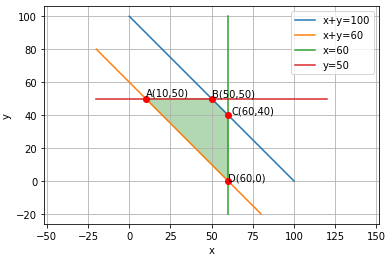
\includegraphics[width=\columnwidth]{graphical solution.PNG}
\caption{Graphical Solution}
\label{fig:Graphical Solution}	
\end{figure}
\end{document}









\end{document}
